\documentclass[11pt,a4paper]{article}
\usepackage{gtu-el-yazisi}
\begin{document}
\notbilgi{İşaretler ve Sistemler}{Ders 12 -- Laplace Transformu}{Isaret-ve-Sistemler-ders-12.pdf}
\providecommand{\yalti}[1]{{\color{yesilkalem}\underline{\color{murekkep}#1}}}

\section{Laplace Transformu}
\sayfa{1}
\begin{align*}
  &X(s)=\int_{-\infty}^{\infty}x(t)e^{-st}\,dt\\
  &x(t)\ \overset{\mathcal{L}}{\longleftrightarrow}\ X(s)\\
  &X(s)=\mathcal{L}\{x(t)\}
\end{align*}
\[
  \Rightarrow s=\sigma+j\omega\ \
  \begin{array}{l}
    \longrightarrow \sigma:\ \text{Reel kısım}\\
    \hookrightarrow \omega:\ \text{Sanal kısım}
  \end{array}
\]
\[
  X(\sigma+j\omega)=\int_{-\infty}^{\infty}x(t)e^{-(\sigma+j\omega)t}\,dt=\int_{-\infty}^{\infty}x(t)e^{-\sigma t}e^{-j\omega t}\,dt=\mathcal{F}\bigl\{x(t)e^{-\sigma t}\bigr\}
\]
$\Rightarrow s=j\omega$
\[
  X(j\omega)=\int_{-\infty}^{\infty}x(t)e^{-j\omega t}\,dt=\mathcal{F}\{x(t)\}=X(s)\Big|_{s=j\omega}
\]
Laplace transformu, $x(t)e^{-\sigma t}$ şeklinde $x(t)$ işaretinin bir reel üstel işaret ile çarpımının Fourier transformudur.
\[
  e^{-\sigma t}\ \
  \begin{array}{l}
    \longrightarrow \sigma>0\ \ \text{zamanla azalan fonksiyon}\\
    \hookrightarrow \sigma<0\ \ \text{zamanla artan fonksiyon}
  \end{array}
\]

\begin{ornek}[]
  $x(t)=e^{-at}\yalti{u(t)}$
\end{ornek}
\[
  X(s)=\int_{-\infty}^{\infty}x(t)e^{-st}\,dt=\int_{-\infty}^{\infty}e^{-at}u(t)e^{-st}\,dt=\int_{0}^{\infty}e^{-(a+s)t}\,dt
  =\frac{e^{-(a+s)t}}{-(a+s)}\bigg|_0^{\infty}=\yalti{\dfrac{1}{s+a}},\ \ \yalti{\mathrm{Re}\{s+a\}>0}
\]
\begin{align*}
  s=\sigma+j\omega&\longrightarrow X(\sigma+j\omega)=\frac{1}{(\sigma+a)+j\omega},\ \ \sigma+a>0\\
  s=j\omega,\ \sigma=0&\longrightarrow X(j\omega)=\frac{1}{a+j\omega},\ \ a>0
\end{align*}
\[
  \left.
  \begin{array}{l}
    e^{-at}u(t)\ \overset{\mathcal{L}}{\longleftrightarrow}\ \dfrac{1}{s+a},\ \ \mathrm{Re}\{s\}>\yalti{-a}\\[4mm]
    u(t)\ \overset{\mathcal{L}}{\longleftrightarrow}\ \dfrac{1}{s},\ \ \mathrm{Re}\{s\}>0
  \end{array}
  \right)\ a=0
\]

\begin{ornek}[]
  $x(t)=-e^{-at}u(-t)$
\end{ornek}
\[
  X(s)=\int_{-\infty}^{\infty}x(t)e^{-st}\,dt=-\int_{-\infty}^{\infty}e^{-at}u(-t)e^{-st}\,dt=-\int_{-\infty}^{0}e^{-(a+s)t}\,dt=\frac{1}{s+a},\ \ \mathrm{Re}\{s+a\}<0
\]
\[
  -e^{-at}u(-t)\ \overset{\mathcal{L}}{\longleftrightarrow}\ \frac{1}{s+a},\ \ \mathrm{Re}\{s\}<-a
\]

\sayfa{2}
$\Rightarrow$ \textbf{Yakınsaklık bölgesi (Region of convergence, ROC):} Laplace transform integralinin yakınsadığı $s$ değer aralığına yakınsaklık bölgesi denir.

\noindent
\begin{minipage}[t]{0.48\linewidth}
  \centering
  \begin{tikzpicture}[scale=0.6]
    \begin{scope}
      \clip (-1,-2) rectangle (3,2.2);
      \foreach \i in {-6,-5.5,...,3} \draw[kursunkalem] (\i,-2) -- ++(4.2,4.2);
    \end{scope}
    \draw[dashed] (-1,-2) -- (-1,2.2);
    \draw[->] (-3.2,0) -- (3.4,0) node[right] {$\sigma$} node[below right] {\scriptsize$\mathrm{Re}\{s\}$};
    \draw[->] (0,-2.2) -- (0,2.6) node[above] {$j\omega$} node[below right] {\scriptsize$\mathrm{Im}\{s\}$};
    \node[below left] at (-1,0) {\scriptsize$-a$};
    \node at (0,-2.7) {$s$-düzlemi};
  \end{tikzpicture}\\[1mm]
  $\mathcal{L}\{e^{-at}u(t)\}=\dfrac{1}{s+a},\ \ \yalti{\mathrm{Re}\{s\}>-a}$
\end{minipage}\hfill
\begin{minipage}[t]{0.48\linewidth}
  \centering
  \begin{tikzpicture}[scale=0.6]
    \begin{scope}
      \clip (-3.2,-2) rectangle (-1,2.2);
      \foreach \i in {-8,-7.5,...,1} \draw[kursunkalem] (\i,-2) -- ++(4.2,4.2);
    \end{scope}
    \draw[dashed] (-1,-2) -- (-1,2.2);
    \draw[->] (-3.2,0) -- (3.4,0) node[right] {$\sigma$};
    \draw[->] (0,-2.2) -- (0,2.6) node[above] {$j\omega$};
    \node[below right] at (-1,0) {\scriptsize$-a$};
    \node at (0,-2.7) {$s$-düzlemi};
  \end{tikzpicture}\\[1mm]
  $\mathcal{L}\{-e^{-at}\yalti{u(-t)}\}=\dfrac{1}{s+a},\ \ \mathrm{Re}\{s\}<-a$
\end{minipage}

\begin{ornek}[]
  $x(t)=\yalti{3e^{-2t}u(t)-2e^{-t}u(t)}$
\end{ornek}
\[
  \left.
  \begin{array}{l}
    e^{-2t}u(t)\ \overset{\mathcal{L}}{\longleftrightarrow}\ \dfrac{1}{s+2},\ \ \mathrm{Re}\{s\}>-2\\[4mm]
    e^{-t}u(t)\ \longleftrightarrow\ \dfrac{1}{s+1},\ \ \mathrm{Re}\{s\}>-1
  \end{array}
  \ \right)
\]
\[
  X(s)=\frac{3}{s+2}-\frac{2}{s+1}=\frac{s-1}{s^2+3s+2},\ \ \mathrm{Re}\{s\}>-1
\]
\noindent
\begin{minipage}[c]{0.45\linewidth}
  \centering
  \begin{tikzpicture}[scale=0.6]
    \begin{scope}
      \clip (-1,-2) rectangle (2.6,2.2);
      \foreach \i in {-6,-5.5,...,3} \draw[kursunkalem] (\i,-2) -- ++(4.2,4.2);
    \end{scope}
    \draw[->] (-3.2,0) -- (3.4,0) node[right] {Re};
    \draw[->] (0,-2.2) -- (0,2.6) node[above] {Im};
    \foreach \p in {-2,-1} \node[thick] at (\p,0) {$\times$};
    \draw[thick] (1,0) circle (0.13);
    \node[below] at (-2,-0.1) {\scriptsize$-2$};
    \node[below] at (-1,-0.1) {\scriptsize$-1$};
    \node[below] at (1,-0.1) {\scriptsize$1$};
    \node at (0,-2.7) {$s$-düzlemi};
  \end{tikzpicture}
\end{minipage}\hfill
\begin{minipage}[c]{0.52\linewidth}
  $\times$: pole (root of denumerator) \ {\small(kutup)}\\[1mm]
  $\circ$: zero (root of numerator) \ {\small(sıfır)}
\end{minipage}

\begin{ornek}[]
  $x(t)=\delta(t)-\frac43e^{-t}u(t)+\frac12e^{2t}u(t)$
\end{ornek}
\[
  \mathcal{L}\{\delta(t)\}=\int_{-\infty}^{\infty}\delta(t)e^{-st}\,dt=\int_{-\infty}^{\infty}\delta(t)e^{-s0}\,dt=\int_{-\infty}^{\infty}\delta(t)\,dt=1
\]
\begin{align*}
  \delta(t)\ &\overset{\mathcal{L}}{\longleftrightarrow}\ 1,\ \ \forall s\ \ (\text{ROC, bütün } s\text{-düzlemi})\\
  e^{-t}u(t)\ &\overset{\mathcal{L}}{\longleftrightarrow}\ \frac{1}{s+1},\ \ \mathrm{Re}\{s\}>-1\\
  e^{2t}u(t)\ &\longleftrightarrow\ \frac{1}{s-2},\ \ \mathrm{Re}\{s\}>2
\end{align*}
\[
  X(s)=1-\frac43\,\frac{1}{s+1}+\frac12\,\frac{1}{s-2}=\frac{(s-1)^2}{(s+1)(s-2)},\ \ \mathrm{Re}\{s\}>2\text{\footnotemark}
\]
\footnotetext{Claude notu: $\frac12$ katsayısıyla toplam $\dfrac{s^2-\frac{11}{6}s+\frac76}{(s+1)(s-2)}$ olur; $\dfrac{(s-1)^2}{(s+1)(s-2)}$ sonucu katsayı $\frac13$ iken elde edilir (muhtemelen $x(t)$'de $\frac13e^{2t}u(t)$ olmalı).}

\sayfa{3}
\begin{center}
  \begin{tikzpicture}[scale=0.6]
    \begin{scope}
      \clip (2,-2) rectangle (4.4,2.2);
      \foreach \i in {-3,-2.5,...,5} \draw[kursunkalem] (\i,-2) -- ++(4.2,4.2);
    \end{scope}
    \draw[dashed] (2,-2) -- (2,2.2);
    \draw[->] (-3,0) -- (4.8,0) node[right] {Re};
    \draw[->] (0,-2.2) -- (0,2.6) node[above] {Im};
    \foreach \p in {-1,2} \node[thick] at (\p,0) {$\times$};
    \draw[thick] (1,0) circle (0.13); \draw[thick] (1,0) circle (0.24);
    \node[below] at (-1,-0.1) {\scriptsize$-1$};
    \node[below] at (1,-0.2) {\scriptsize$1$};
    \node[below right] at (2,-0.1) {\scriptsize$2$};
  \end{tikzpicture}
\end{center}
$\Rightarrow$ Aynı noktada tekrar eden $s$ sayısına mertebe denir.\\
Paydada, $s=-1$ ve $s=2$ olmak üzere birinci mertebeden iki adet kutup ve payda $s=1$'de ikinci mertebeden bir adet sıfır vardır.

\medskip
\textbf{Not:} Laplace transformunun ROC'u $j\omega$ eksenini içermiyorsa Fourier transformu yakınsamaz.\\
$\frac13e^{2t}u(t)$ ifadesinin Fourier transformu yoktur.

\subsection{Yakınsama bölgesi (ROC) özellikleri}
\begin{enumerate}[label=\arabic*)]
  \item $X(s)$'in ROC'u $s$-düzlemindeki $j\omega$ eksenine paralel şeritlerden oluşur.
    \[
      X(s)\underset{\substack{\uparrow\\ s=\sigma+j\omega}}{=}X(\sigma+j\omega)=\int_{-\infty}^{\infty}x(t)e^{-st}\,dt=\int_{-\infty}^{\infty}x(t)e^{-\sigma t}e^{-j\omega t}\,dt=\mathcal{F}\bigl\{\yalti{x(t)e^{-\sigma t}}\bigr\}
    \]
    \[ \int_{-\infty}^{\infty}|x(t)|e^{-\sigma t}\,dt\ \yalti{<\infty} \]
  \item Rasyonel Laplace transform için, ROC herhangi bir kutup içermez.
  \item $x(t)$ sonlu süreli ve mutlak entegre edilebilir ise, ROC bütün $s$ düzlemidir.
    \begin{align*}
      &\int_{T_1}^{T_2}|x(t)|\,dt<\infty\\
      &\int_{T_1}^{T_2}|x(t)|e^{-\sigma t}\,dt<\infty\ \longleftarrow\ \text{1) özellik}
    \end{align*}
    $\rightarrow$ $\mathrm{Re}\{s\}=\sigma=0$ iken $s=j\omega$ olup ROC içinde kalır.\\
    $\rightarrow$ $\mathrm{Re}\{s\}=\sigma>0$ iken
    $\displaystyle\int_{T_1}^{T_2}|x(t)|e^{-\sigma t}\,dt<e^{-\sigma T_1}\underbrace{\int_{T_1}^{T_2}|x(t)|\,dt}_{\infty}<\infty$
    olur ve $\mathrm{Re}\{s\}>0$ $s$-düzlemi ROC içinde kalır.\\
    $\rightarrow$ $\mathrm{Re}\{s\}=\sigma<0$ iken
    $\displaystyle\int_{T_1}^{T_2}|x(t)|e^{-\sigma t}\,dt<e^{-\sigma T_2}\int_{T_1}^{T_2}|x(t)|\,dt<\infty$
    olur ve $\mathrm{Re}\{s\}<0$ $s$-düzlemi ROC içinde kalır.
\end{enumerate}

\begin{ornek}[]
  $x(t)=\begin{cases}e^{-at}, & 0<t<T\\ 0, & \text{dışında}\end{cases}$
\end{ornek}
\[
  X(s)=\int_{-\infty}^{\infty}x(t)e^{-st}\,dt=\int_{0}^{T}e^{-(a+s)t}\,dt=\frac{1}{s+a}\Bigl(1-e^{-(a+s)T}\Bigr)\ \longleftarrow
\]
\begin{flushright}
  3)'e göre ROC bütün $s$ düzlemi\\
  2)'e göre ROC kutup içermez, $s=-a$ kutup var.
\end{flushright}
$s=-a$ iken $X(s)=\dfrac00$

\sayfa{4}
\[
  \lim_{s\to-a}X(s)=\lim_{s\to-a}\left(\frac{\frac{d}{ds}\bigl(1-e^{-(a+s)T}\bigr)}{\frac{d}{ds}(s+a)}\right)=\lim_{s\to-a}Te^{-aT}e^{-sT}
  \ \Longrightarrow\ \yalti{X(-a)=T}
\]
\begin{enumerate}[label=\arabic*), start=4]
  \item $x(t)$ sağ yönlü ve $\mathrm{Re}\{s\}=\sigma_0$ doğrusu ROC'da ise, $\yalti{\mathrm{Re}\{s\}>\sigma_0}$ için bütün $s$ değerleri de ROC'da olur.\par
    \begin{tikzpicture}[scale=0.55]
      \draw[->] (-2.5,0) -- (3.5,0) node[right] {$t$};
      \draw[->] (0,-0.2) -- (0,1.8) node[above] {$x(t)$};
      \draw[murekkep, thick] (-2.5,0) -- (-1.2,0) -- (-1.2,0.6);
      \draw[murekkep, thick, smooth] plot[domain=-1.2:3, samples=60] (\x, {0.6+0.15*sin(deg(3*\x))+0.1*sin(deg(5*\x+1))});
    \end{tikzpicture}\hspace{1.5cm}
    \begin{tikzpicture}[scale=0.55]
      \begin{scope}
        \clip (-0.7,-1.6) rectangle (2.2,1.8);
        \foreach \i in {-5,-4.5,...,3} \draw[kursunkalem] (\i,-1.6) -- ++(3.4,3.4);
      \end{scope}
      \draw[dashed] (-0.7,-1.6) -- (-0.7,1.8);
      \draw[->] (-2.4,0) -- (2.6,0) node[right] {Re};
      \draw[->] (0,-1.6) -- (0,2.1) node[above] {Im};
      \node[below left] at (-0.7,0) {\scriptsize$\sigma_0$};
    \end{tikzpicture}
  \item $x(t)$ sol yönlü ve $\mathrm{Re}\{s\}=\sigma_0$ doğrusu ROC'da ise, $\mathrm{Re}\{s\}<\sigma_0$ için bütün $s$ değerleri de ROC'da olur.\par
    \begin{tikzpicture}[scale=0.55]
      \draw[->] (-3.5,0) -- (2.5,0) node[right] {$t$};
      \draw[->] (0,-0.2) -- (0,1.8) node[above] {$x(t)$};
      \draw[murekkep, thick, smooth] plot[domain=-3.2:0.9, samples=60] (\x, {0.7+0.15*sin(deg(3*\x))+0.1*sin(deg(5*\x+1))});
      \draw[murekkep, thick] (0.9,{0.7+0.15*sin(deg(2.7))+0.1*sin(deg(5.5))}) -- (0.9,0) -- (2.2,0);
    \end{tikzpicture}\hspace{1.5cm}
    \begin{tikzpicture}[scale=0.55]
      \begin{scope}
        \clip (-2.2,-1.6) rectangle (0.7,1.8);
        \foreach \i in {-6,-5.5,...,1} \draw[kursunkalem] (\i,-1.6) -- ++(3.4,3.4);
      \end{scope}
      \draw[dashed] (0.7,-1.6) -- (0.7,1.8);
      \draw[->] (-2.4,0) -- (2.6,0) node[right] {Re};
      \draw[->] (0,-1.6) -- (0,2.1) node[above] {Im};
      \node[below right] at (0.7,0) {\scriptsize$\sigma_0$};
    \end{tikzpicture}
  \item $x(t)$ çift yönlü ve $\mathrm{Re}\{s\}=\sigma_0$ doğrusu ROC'da ise, ROC, $s$ düzleminde $\mathrm{Re}\{s\}=\sigma_0$ doğrusunu içeren bir şeritten oluşur.\par
    \begin{tikzpicture}[scale=0.55]
      \draw[->] (-3.5,0) -- (3.5,0) node[right] {$t$};
      \draw[->] (0,-0.2) -- (0,1.8) node[above] {$x(t)$};
      \draw[murekkep, thick, smooth] plot[domain=-3.2:3.2, samples=80] (\x, {0.5+0.6*exp(-1.5*abs(\x))+0.1*sin(deg(3*\x))});
    \end{tikzpicture}\hspace{1.5cm}
    \begin{tikzpicture}[scale=0.55]
      \begin{scope}
        \clip (-0.9,-1.6) rectangle (0.9,1.8);
        \foreach \i in {-5,-4.5,...,2} \draw[kursunkalem] (\i,-1.6) -- ++(3.4,3.4);
      \end{scope}
      \draw[dashed] (-0.9,-1.6) -- (-0.9,1.8);
      \draw[dashed] (0.9,-1.6) -- (0.9,1.8);
      \draw[->] (-2.4,0) -- (2.6,0) node[right] {Re};
      \draw[->] (0,-1.6) -- (0,2.1) node[above] {Im};
      \node[below left] at (-0.9,0) {\scriptsize$\sigma_R$};
      \node[below right] at (0.9,0) {\scriptsize$\sigma_L$};
    \end{tikzpicture}
  \item $X(s)$ rasyonel ise, ROC, ya kutuplarla sınırlıdır ya da sonsuza genişler ve kutup içermez.\\
    $\rightarrow$ $x(t)$ sağ yönlü ise, ROC, en sağdaki kutubun sağında kalan $s$ düzlemidir.\\
    $\rightarrow$ $x(t)$ sol yönlü ise, ROC en soldaki kutubun solunda kalan $s$ düzlemidir.
\end{enumerate}

\begin{ornek}[]
  $x(t)=e^{-b|t|}$
\end{ornek}
\[
  X(s)=\int_{-\infty}^{\infty}x(t)e^{-st}\,dt=\int_{-\infty}^{0}e^{bt}e^{-st}\,dt+\int_{0}^{\infty}e^{-bt}e^{-st}\,dt
  =\frac{-1}{\yalti{s-b}}+\frac{1}{\yalti{s+b}},\qquad
  \begin{array}{l}\mathrm{Re}\{s-b\}<0\\ \mathrm{Re}\{s+b\}>0\end{array}
\]
\[
  X(s)=\frac{-2b}{s^2-b^2},\qquad -b<\mathrm{Re}\{s\}<b
\]
\begin{center}
  \begin{tikzpicture}[scale=0.6]
    \draw[->] (-3.6,0) -- (3.8,0) node[right] {$t$};
    \draw[->] (0,-0.2) -- (0,2.4) node[above right] {$x(t)=e^{-b|t|},\ b>0$};
    \draw[murekkep, thick, smooth] plot[domain=-3.4:3.4, samples=81] (\x, {1.6*exp(-abs(\x))});
    \node[above right] at (0,1.6) {\scriptsize$1$};
  \end{tikzpicture}\hspace{1.5cm}
  \begin{tikzpicture}[scale=0.6]
    \begin{scope}
      \clip (-1,-1.8) rectangle (1,2);
      \foreach \i in {-5,-4.5,...,2} \draw[kursunkalem] (\i,-1.8) -- ++(3.8,3.8);
    \end{scope}
    \draw[dashed] (-1,-1.8) -- (-1,2); \draw[dashed] (1,-1.8) -- (1,2);
    \draw[->] (-2.6,0) -- (2.8,0) node[right] {Re};
    \draw[->] (0,-1.8) -- (0,2.3) node[above] {Im};
    \node at (-1,0) {$\times$}; \node at (1,0) {$\times$};
    \node[below left] at (-1,-0.1) {\scriptsize$-b$};
    \node[below right] at (1,-0.1) {\scriptsize$b$};
  \end{tikzpicture}
\end{center}

\sayfa{5}
\begin{ornek}[]
  $X(s)=\dfrac{1}{(s+1)(s+2)}=\dfrac{1}{s+1}-\dfrac{1}{s+2}$
\end{ornek}
\noindent
\begin{minipage}[t]{0.32\linewidth}
  \centering
  \begin{tikzpicture}[scale=0.5]
    \begin{scope}
      \clip (-1,-1.8) rectangle (2.2,2);
      \foreach \i in {-5,-4.5,...,3} \draw[kursunkalem] (\i,-1.8) -- ++(3.8,3.8);
    \end{scope}
    \draw[dashed] (-1,-1.8) -- (-1,2);
    \draw[->] (-2.8,0) -- (2.5,0) node[right] {Re};
    \draw[->] (0,-1.8) -- (0,2.3) node[above] {Im};
    \node at (-2,0) {$\times$}; \node at (-1,0) {$\times$};
    \node[below] at (-2,-0.1) {\scriptsize$-2$}; \node[below] at (-1,-0.1) {\scriptsize$-1$};
  \end{tikzpicture}\\[1mm]
  \raggedright
  $x(t)$ sağ yönlü ise\\[1mm]
  $x(t)=e^{-t}u(t)-e^{-2t}u(t)$\\[1mm]
  ROC, $s=j\omega$ içerir, FT yakınsar.
\end{minipage}\hfill
\begin{minipage}[t]{0.32\linewidth}
  \centering
  \begin{tikzpicture}[scale=0.5]
    \begin{scope}
      \clip (-2.8,-1.8) rectangle (-2,2);
      \foreach \i in {-8,-7.5,...,0} \draw[kursunkalem] (\i,-1.8) -- ++(3.8,3.8);
    \end{scope}
    \draw[dashed] (-2,-1.8) -- (-2,2);
    \draw[->] (-2.8,0) -- (2.5,0) node[right] {Re};
    \draw[->] (0,-1.8) -- (0,2.3) node[above] {Im};
    \node at (-2,0) {$\times$}; \node at (-1,0) {$\times$};
    \node[below] at (-2,-0.1) {\scriptsize$-2$}; \node[below] at (-1,-0.1) {\scriptsize$-1$};
  \end{tikzpicture}\\[1mm]
  \raggedright
  $x(t)$ sol yönlü ise\\[1mm]
  $x(t)=-e^{-t}u(-t)+e^{-2t}u(-t)$\\[1mm]
  FT yoktur
\end{minipage}\hfill
\begin{minipage}[t]{0.32\linewidth}
  \centering
  \begin{tikzpicture}[scale=0.5]
    \begin{scope}
      \clip (-2,-1.8) rectangle (-1,2);
      \foreach \i in {-7,-6.5,...,0} \draw[kursunkalem] (\i,-1.8) -- ++(3.8,3.8);
    \end{scope}
    \draw[dashed] (-2,-1.8) -- (-2,2); \draw[dashed] (-1,-1.8) -- (-1,2);
    \draw[->] (-2.8,0) -- (2.5,0) node[right] {Re};
    \draw[->] (0,-1.8) -- (0,2.3) node[above] {Im};
    \node at (-2,0) {$\times$}; \node at (-1,0) {$\times$};
    \node[below] at (-2,-0.1) {\scriptsize$-2$}; \node[below] at (-1,-0.1) {\scriptsize$-1$};
  \end{tikzpicture}\\[1mm]
  \raggedright
  $x(t)$ çift yönlü ise\\[1mm]
  $x(t)=-e^{-t}u(-t)-e^{-2t}u(t)$\\[1mm]
  FT yoktur.
\end{minipage}

\subsection{Ters Laplace Transform}
\begin{align*}
  X(s)&=X(\sigma+j\omega)=\int_{-\infty}^{\infty}x(t)e^{-\sigma t}e^{-{\color{yesilkalem}j\omega}t}\,dt=\mathcal{F}\bigl\{\yalti{x(t)e^{-\sigma t}}\bigr\}\\
  \yalti{x(t)e^{-\sigma t}}&=\mathcal{F}^{-1}\{X(\sigma+j\omega)\}=\frac{1}{2\pi}\int_{-\infty}^{\infty}X(\sigma+j\omega)e^{j\omega t}\,d\omega\\
  x(t)&=\frac{1}{2\pi}\int_{-\infty}^{\infty}X(\yalti{\sigma+j\omega})e^{(\sigma+j\omega)t}\,\yalti{d\omega}
\end{align*}
\[ s=\sigma+j\omega\ \longrightarrow\ ds=j\,d\omega \]
\formulkutu{x(t)=\frac{1}{2\pi j}\int_{\sigma-j\infty}^{\sigma+j\infty}X(s)e^{st}\,ds}
\[
  \Rightarrow X(s)=\sum_{i=1}^{m}\frac{A_i}{s+a_i}\ \
  \begin{array}{l}
    \longrightarrow x(t)=A_ie^{-a_it}u(t)\ :\ \text{sağ yönlü}\\[1mm]
    \hookrightarrow x(t)=-A_ie^{-a_it}u(-t)\ :\ \text{sol yönlü}
  \end{array}
\]

\section{Laplace Transformunun Özellikleri}
\[
  x(t)\ \overset{\mathcal{L}}{\longleftrightarrow}\ X(s),\ \ \text{ROC}: R
  \qquad\qquad
  X(s)=\mathcal{L}\{x(t)\}\qquad x(t)=\mathcal{L}^{-1}\{X(s)\}
\]
\begin{enumerate}[label=\arabic*)]
  \item \textbf{Lineerlik:} \ $\alpha x_1(t)+\beta x_2(t)\ \longleftrightarrow\ \alpha X_1(s)+\beta X_2(s)$, \ ROC: $R_1\cap R_2$
  \item \textbf{Zamanda öteleme:} \ $x(t-t_0)\ \longleftrightarrow\ e^{-st_0}X(s)$, \ ROC: $R$
  \item \textbf{$s$-domeninde öteleme:} \ $e^{s_0t}x(t)\ \longleftrightarrow\ X(s-s_0)$, \ ROC: $R+\mathrm{Re}\{s_0\}$\\
    $s_0=j\omega_0\ \Rightarrow\ e^{j\omega_0t}x(t)\ \longleftrightarrow\ X(s-j\omega_0)$, \ ROC: $R$
  \item \textbf{Zamanda ölçeklendirme:} \ $x(at)\ \longleftrightarrow\ \dfrac{1}{|a|}X(s/a)$, \ ROC: $R/a$\\
    $a=-1\ \Rightarrow\ x(-t)=X(-s)$, \ ROC: $-R$
  \item \textbf{Eşlenik alma:} \ $x^*(t)\ \longleftrightarrow\ X^*(s^*)$, \ ROC: $R$
  \item \textbf{Türev:} \ $\dfrac{dx(t)}{dt}\ \longleftrightarrow\ sX(s)$, \ ROC: $R$'yi içerir.\\[1mm]
    \phantom{\textbf{Türev:} \ }$-t\,x(t)\ \longleftrightarrow\ \dfrac{dX(s)}{ds}$, \ ROC: $R$
  \sayfa{6}
  \item \textbf{Integral:} \ $\displaystyle\int_{-\infty}^{t}x(\tau)\,d\tau\ \longleftrightarrow\ \frac1sX(s)$, \ ROC: $R\cap\{\mathrm{Re}\{s\}>0\}$
  \item \textbf{Konvolüsyon:} \ $x_1(t)*x_2(t)\ \longleftrightarrow\ X_1(s)X_2(s)$, \ $\yalti{\text{ROC}: R_1\cap R_2}$
    \begin{center}
      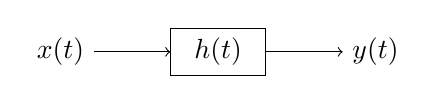
\begin{tikzpicture}
        \node (x) at (0,0) {$x(t)$};
        \node[draw, rectangle, minimum width=1.2cm, minimum height=0.6cm] (h) at (2,0) {$h(t)$};
        \node (y) at (4,0) {$y(t)$};
        \draw[->] (x) -- (h); \draw[->] (h) -- (y);
      \end{tikzpicture}
    \end{center}
    \[
      y(t)=x(t)\,\yalti{*}\,h(t)\ \longleftrightarrow\
      \begin{array}{l}
        Y(s)=X(s)H(s)\\[1mm]
        H(s)=\dfrac{Y(s)}{X(s)}\ :\ \text{Transfer fonksiyonu}
      \end{array}
    \]
\end{enumerate}

\begin{ornek}[]
  $x(t)=t\,e^{-at}u(t)$, \ $X(s)=\,?$
\end{ornek}
\begin{align*}
  {\color{yesilkalem}t}\,\yalti{e^{-at}u(t)\ \longleftrightarrow\ \frac{1}{s+a},\ \ \mathrm{Re}\{s\}>-a}\\[2mm]
  t\,e^{-at}u(t)\ &\longleftrightarrow\ {\color{yesilkalem}-}\frac{d}{ds}\Bigl(\frac{1}{s+a}\Bigr)=\frac{1}{(s+a)^2},\ \ \yalti{\mathrm{Re}\{s\}>-a}\\
  \frac{t^2}{2}e^{-at}u(t)\ &\longleftrightarrow\ \frac{1}{(s+a)^3},\ \ \mathrm{Re}\{s\}>-a\\
  &\ \ \vdots\\
  \frac{t^{n-1}}{(n-1)!}e^{-at}u(t)\ &\longleftrightarrow\ \frac{1}{(s+a)^n},\ \ \mathrm{Re}\{s\}>-a
\end{align*}

\begin{ornek}[]
  $H(s)=\dfrac{2s^2+5s+5}{(s+1)^2(s+2)}$, \ $\mathrm{Re}\{s\}>-1$, \ $h(t)=\,?$
\end{ornek}
\[
  H(s)=\frac{A}{(s+1)^2}+\frac{B}{(s+1)}+\frac{C}{(s+2)}\ \longrightarrow\
  \begin{array}{l} A=2\\ B=-1\\ C=3\end{array}
\]
\[ \Big\updownarrow\,\mathcal{L}^{-1} \]
\[
  h(t)=2te^{-t}u(t)-e^{-t}u(t)+3e^{-2t}u(t)
\]

\section{ROC ile LTI sistemlerin özelliklerinin analizi}
\begin{enumerate}[label=\arabic*)]
  \item \textbf{Nedensellik:} \ $h(t)=0,\ t<0$ \ sağ yönlü $\longrightarrow$ ROC sağ yönlü
  \item \textbf{Kararlılık:} \ $\displaystyle\int_{-\infty}^{\infty}|h(t)|\,dt<\infty\ \longrightarrow$ ROC, $j\omega$ eksenini içermelidir.
\end{enumerate}

\sayfa{7}
\begin{ornek}[]
  $h(t)=e^{-t}\yalti{u(t)}$, \ kararlı mıdır?
\end{ornek}
\noindent
\begin{minipage}[c]{0.55\linewidth}
  \[ \Big\updownarrow \]
  \[ H(s)=\frac{1}{s+1},\ \ \mathrm{Re}\{s\}>-1 \]
  ROC sağ yönlü olduğundan nedenseldir.
\end{minipage}\hfill
\begin{minipage}[c]{0.4\linewidth}
  \centering
  \begin{tikzpicture}[scale=0.5]
    \begin{scope}
      \clip (-1,-1.8) rectangle (2.2,2);
      \foreach \i in {-5,-4.5,...,3} \draw[kursunkalem] (\i,-1.8) -- ++(3.8,3.8);
    \end{scope}
    \draw[dashed] (-1,-1.8) -- (-1,2);
    \draw[->] (-2.4,0) -- (2.6,0) node[right] {Re};
    \draw[->] (0,-1.8) -- (0,2.3) node[above] {Im};
    \node at (-1,0) {$\times$};
    \node[below left] at (-1,-0.1) {\scriptsize$-1$};
  \end{tikzpicture}
\end{minipage}

\begin{ornek}[]
  $h(t)=e^{-|t|}\ \longleftrightarrow\ H(s)=\dfrac{-2}{s^2-1}$, \ $-1<\mathrm{Re}\{s\}<1$
\end{ornek}
\begin{center}
  \begin{tikzpicture}[scale=0.5]
    \begin{scope}
      \clip (-1,-1.8) rectangle (1,2);
      \foreach \i in {-5,-4.5,...,2} \draw[kursunkalem] (\i,-1.8) -- ++(3.8,3.8);
    \end{scope}
    \draw[dashed] (-1,-1.8) -- (-1,2); \draw[dashed] (1,-1.8) -- (1,2);
    \draw[->] (-2.4,0) -- (2.6,0) node[right] {Re};
    \draw[->] (0,-1.8) -- (0,2.3) node[above] {Im};
    \node[below left] at (-1,-0.1) {\scriptsize$-1$};
    \node[below right] at (1,-0.1) {\scriptsize$1$};
  \end{tikzpicture}
  \qquad Nedensel değildir.
\end{center}

\begin{ornek}[]
  $H(s)=\dfrac{s-1}{(s+1)(s-2)}=\dfrac{A}{s+1}+\dfrac{B}{s-2}$, \qquad $A=2/3$, \ $B=\dfrac13$
\end{ornek}
\noindent
\begin{minipage}[t]{0.32\linewidth}
  \centering
  \begin{tikzpicture}[scale=0.45]
    \begin{scope}
      \clip (2,-1.8) rectangle (3.4,2);
      \foreach \i in {-3,-2.5,...,4} \draw[kursunkalem] (\i,-1.8) -- ++(3.8,3.8);
    \end{scope}
    \draw[dashed] (2,-1.8) -- (2,2);
    \draw[->] (-2,0) -- (3.6,0) node[right] {Re};
    \draw[->] (0,-1.8) -- (0,2.3) node[above] {Im};
    \node at (-1,0) {$\times$}; \node at (2,0) {$\times$}; \draw (1,0) circle (0.15);
    \node[below] at (-1,-0.1) {\scriptsize$-1$}; \node[below] at (1,-0.1) {\scriptsize$1$}; \node[below left] at (2,-0.1) {\scriptsize$2$};
  \end{tikzpicture}\\
  \raggedright\small
  $h(t)$ sağ yönlü\\[1mm]
  $h(t)=\frac23e^{-t}u(t)+\frac13e^{2t}u(t)$\\[1mm]
  Nedensel (sağ yönlü)\\
  Kararlı değil ($j\omega$ eksenini içermez)
\end{minipage}\hfill
\begin{minipage}[t]{0.32\linewidth}
  \centering
  \begin{tikzpicture}[scale=0.45]
    \begin{scope}
      \clip (-2,-1.8) rectangle (-1,2);
      \foreach \i in {-7,-6.5,...,0} \draw[kursunkalem] (\i,-1.8) -- ++(3.8,3.8);
    \end{scope}
    \draw[dashed] (-1,-1.8) -- (-1,2);
    \draw[->] (-2,0) -- (3.6,0) node[right] {Re};
    \draw[->] (0,-1.8) -- (0,2.3) node[above] {Im};
    \node at (-1,0) {$\times$}; \node at (2,0) {$\times$}; \draw (1,0) circle (0.15);
    \node[below] at (-1,-0.1) {\scriptsize$-1$}; \node[below] at (1,-0.1) {\scriptsize$1$}; \node[below] at (2,-0.1) {\scriptsize$2$};
  \end{tikzpicture}\\
  \raggedright\small
  $h(t)$ sol yönlü\\[1mm]
  $h(t)=-\frac23e^{-t}u(-t)-\frac13e^{2t}u(-t)$\\[1mm]
  Nedensel değil (sol yönlü)\\
  Kararlı değil
\end{minipage}\hfill
\begin{minipage}[t]{0.32\linewidth}
  \centering
  \begin{tikzpicture}[scale=0.45]
    \begin{scope}
      \clip (-1,-1.8) rectangle (2,2);
      \foreach \i in {-6,-5.5,...,2} \draw[kursunkalem] (\i,-1.8) -- ++(3.8,3.8);
    \end{scope}
    \draw[dashed] (-1,-1.8) -- (-1,2); \draw[dashed] (2,-1.8) -- (2,2);
    \draw[->] (-2,0) -- (3.6,0) node[right] {Re};
    \draw[->] (0,-1.8) -- (0,2.3) node[above] {Im};
    \node at (-1,0) {$\times$}; \node at (2,0) {$\times$}; \draw (1,0) circle (0.15);
    \node[below left] at (-1,-0.1) {\scriptsize$-1$}; \node[below] at (1,-0.1) {\scriptsize$1$}; \node[below right] at (2,-0.1) {\scriptsize$2$};
  \end{tikzpicture}\\
  \raggedright\small
  $h(t)$ çift yönlü\\[1mm]
  $h(t)=\frac23e^{-t}u(t)-\frac13e^{2t}u(-t)$\\[1mm]
  Nedensel değil\\
  Kararlı
\end{minipage}

\begin{ornek}[]
  $\dfrac{d^2y(t)}{dt^2}+3\dfrac{dy(t)}{dt}+2y(t)=\dfrac{dx(t)}{dt}+3x(t)$, \quad $\yalti{h(t)=\,?}$
\end{ornek}
\[ \Big\updownarrow\,\mathcal{L} \]
\[ s^2Y(s)+3sY(s)+2Y(s)=sX(s)+3X(s) \]
\[
  H(s)=\frac{Y(s)}{X(s)}=\frac{s+3}{s^2+3s+2}=\frac{A}{s+1}+\frac{B}{s+2},\qquad
  \begin{array}{l}A=2\\ B=-1\end{array}
\]
\[ \Big\updownarrow\,\mathcal{L}^{-1} \]
\[
  h(t)=2e^{-t}u(t)-e^{-t}u(t),\ \ \mathrm{Re}\{s\}>-1\text{\footnotemark}
\]
\footnotetext{Claude notu: $B/(s+2)$ teriminin ters dönüşümü $e^{-2t}u(t)$'dir; muhtemelen $h(t)=2e^{-t}u(t)-e^{-2t}u(t)$ olmalı.}

\end{document}
